\chapter{Dark Matter}
\lettrine{O}{}ne of the most challenging question of current physics is the nature of Dark Matter. Several evidences discussed in this chapter proves that in the Universe there is non-luminous matter and most of it is of non-baryonic nature. Currently data imply that ordinary matter accounts for about \num{4.56\pm0.16}\% while Dark Matter accounts for \num{22.7\pm1.4}\% and Dark Energy for the remaining \num{72.8\pm1.5}\%.

Dark matter would constitute the principal nonbaryonic contribution to the matter density of the universe. Today DM particles can be produced at collider such LHC if it interacts with Standard Model (SM) particle via couplings at the electroweak scale, On the other hand they certainly cannot be detected but their interaction with the detector is seen as missing energy (\met) defined \textbf{later}. 

\section{The Standard Model of particle physics}
The Standard Model (SM) of particle physics is well established theory of elementary particles and their interaction. Up to now it is considered the most satisfying theory including three of the four fundamental forces.
Particles of SM can be divided into three cathegories. The first comprehend spin \num{1/2} fermions divided in three generations which are the electron, the muon and the $\tau$-lepton with their corresponding neutrinos, along with six flavoured quarks (up, down, strange, charm, top, bottom). The second cathegory includes four spin 0 gauge boson, or the force carriers. They are the photon, mediator of electromagnetic force, the the \Zboson and \Wboson boson mediators of weak force and the gluon which carries strong interation. At last there is the Higgs Boson, whose existence has been proved with \RunOne ATLAS and CMS data.

On the other hand, the SM presents a series of open issues. In addition to major problems such the gauge hierarchy problem, i.e. understand why the Higgs mass is so small compared to the Planck mass, the SM does not contemplate gravitation as a quantum theory nor it provides a particle to be a solid candidate for Dark Matter. There are several extension of the SM trying to include several neutral, stable or at least long lived, and non-baryonic particles that could account for DM constituent.

The principal candidate comes from the so called Weakly Interactive Mass Particles (WIMPs). They are the most studied Dark Matter candidates, since they are found in many particle physics theories, they have the correct relic density, i.e. the measure of the present quantity of a particle remaining from the Big Bang, and may be detected in many ways~\cite{feng:DM}.

Before talking about WIMPs, let's introduce several evidences that justify the search for DM.

\section{Physical evidences of Dark Matter}
In this section num different astronomical observation that rise the idea for non-luminous matter in the Universe and for necessity of physics Beyond Standard Model, are pointed out, starting from gravitational lensing, then discussing the rotation curve of stars in galaxies and finally talking about the Cosmic Microwave Background (CMB).

\subsection{Gravitational lensing}
Gravitational lensing is the phoenomenon for which a very massive object could act as a lens deviating rays of lights. According to general relativity light is affected by gravitational field produced by massive object so that a ray of light could be deflected of an angle 
\begin{equation}
\abs{\delta\phi}=\frac{4M}{b}
\end{equation}
following a potential given by
\begin{equation}
V(r)=\frac{L^2}{2r^3}(1-2M).
\end{equation}

In the prevoius formul\ae $\,M$ is the mass of the object producing the field, $L$ is the angular momentum of the photon, and $b$ is the \emph{apparent} impact parameter defined as $b=L/E$ where $E$ is its energy. Note that we are using a natural system unit in which $G=1$ and $c=1$.

If the light being deflected comes from an object aligned with the lens and the observer and the lens is pefectly homogeneous, the image produces is a perfect circle, like the Einstein ring, since light is deflected equally in every direction. What actually happens is a discrete pattern of images around the lens.

The model used to predict mass for a lens is the singular isothermal sphere (SIS) \cite{book:971430} which approximates the lens as a spherical ideal gas cloud with constant temperature $T$ for every point in the lens. Defining the density of the lens as $\rho(r)=\sigma_v^2/2\pi G r^2$, where $\sigma_v^2$ is the velocity distribution of the lens components along the line-of-sight, the mass within a sphere of radius $r$ is therefore computed as:
\begin{equation}
M(<r)=\int_0^r{\rho(r')4\pi r'^2 dr'}=\frac{2\sigma_v^2}{G}r
\label{mass}
\end{equation}

It is clear that the SIS model is not perfect because, according to \Eqn{\ref{mass}} it gives an infinite total mass, even if it is exploited a lot thanks to its simplicity and its perfect reconstruction of rotation curves of spiral galaxies (\Sect{\ref{sec:rotcurves}}), but further results lie outside of the purpose of this work.

What we want to point out is that  \Eqn{\ref{mass}} accounts for the \emph{total} mass composing the lens, including both luminous and dark. The latter is missed when we try to calculate it from the luminosity of the lens.
   
\subsection{Rotation curves of stars in a galaxy}
\label{sec:rotcurves}
The study of rotation curve of galaxies focuses on spiral galaxies which are bound system where stars are not distributed spherically but in a thin disk. Stars up to a radius $r$ from the center of a galaxy are influenced by innermost others giving the centripetal force to carry the motion. At equilibrium centripetal force must be equal to the gravitational attractive force.
\begin{equation}
\frac{mv^2}{r}=\frac{GM(r)m}{r^2}
\label{previous}
\end{equation}
where $M(r)$ is the mass of the galaxy inside a radius $r$ and $m$ is the mass of a single star. From the previous equation one obtains the velocity distribution:
\begin{equation}
v=\sqrt{\frac{GM(r)}{r}}.
\end{equation}

The theory predicts that velocity should decrease with radius, but actual measurements shows that it remains constant after \SI{\sim5}{pc} as pointed out in data shown in \Fig{\ref{fig:rotation}}. A simple explanation to this behaviour is the presence of a Dark Matter halo throughout the galaxy whose mass distribution is proportional to the distance from the center so that the velocity distribution would be constant.
\begin{figure}[pt]
\centering
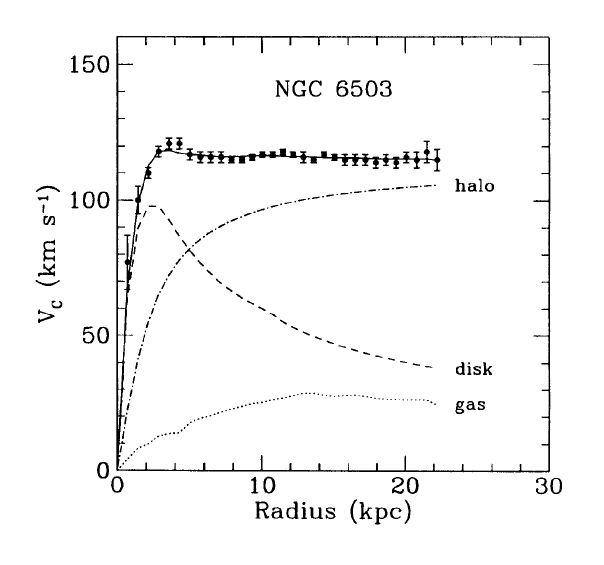
\includegraphics[width=0.5\textwidth]{DarkMatter/Rotationcurves}
\caption{Rotation curves of NGC 6503 galaxy. The image represents a fit on the rotation curves made of three parameters: a stellar (dashed) and a gaseous disk (dotted) and a Dark Matter halo (dash-dotted) modeled by a singular isothermal sphere (SIS).}
\label{fig:rotation}
\end{figure}


\subsection{Cosmic Microwave Background}
The CMB is the residue of the thermal microwave radiation emitted \SI{\sim 3e5} years after the Big Bang, when the Universe became transparent to photons. Before that it was an ionized plasma in which matter and radiation were tightly coupled. So CMB is a footprint of Universe at that moment from which several informations on cosmological parameters of that age can be inferred. One of them is the abundance of DM and Dark Energy. This results were achieved by the PLANCK experiment (ESA), which mapped also the anisotropies of this radiation in universe, according to which the Universe would be composed of ordinary matter for the 5\%, for Dark Matter for the 26\% and Dark Energy for the 69\% \cite{Planck:results}.

\section{The WIMP hypothesis}
\label{sec:wimp}
As mentioned above a WIMP is an hypothetical massive particle that could account for DM. The WIMP miracle states that if a such a particle exists and it is stable it has a relic density consistent with Dark Matter. This implies that particles involved in the electroweak symmetry breaking, with mass in the \SI{10}{\GeV} - \SI{1}{\TeV} range, could be good constitute DM and allows to find the correct order of magnitude for the DM abundance \cite{DMcollider}.

Dark Matter has been produced as thermal relic of the Big Bang and its evolution takes different steps. Initially the early Universe is dense and hot, and all particles are in thermal equilibrium. With its cooling down to a temperature T below the DM mass (if $c=1$ and $k_b=1$) these particle became Boltzmann suppressed. The Universe is also expanding, so that DM particles are going to ``freeze out'' with their number asymptotically approaching a constant (see \Fig{\ref{fig:Freezeout}}): their thermal relic density. This process is described quantitatively by the Boltzmann equation:
\begin{equation}
\frac{dn}{dt}=-3Hn-\avg{\sigma_A v}\left(n^2-n_{\textup{eq}}^2\right)
\label{eqn:boltz}
\end{equation}

where $n$ is the number density of the dark matter particle $H$ is the Hubble parameter, \avg{\sigma_A v} is the thermally averaged annihilation cross section, and $n_{\textup{eq}}$ is is the dark matter number density in thermal equilibrium \cite{feng:DM}. Solving \Eqn{\ref{eqn:boltz}}, numerically, the thermal relic density is determined. Moreover we can define the freeze out time when the Hubble parameter became important, i.e. $n\avg{\sigma_A v}= H$, at that time, the number density stopped changing and that is the relic abundance of Dark Matter we observe today.

In formul\ae, where $f$ subscript denotes quantities at thermal freeze out and $0$ present day quantity, we have:
\begin{equation}
	n_f\simeq\frac{T^2_f}{M_\textup{Pl}\avg{\sigma_A v}}
\end{equation}
where $M_\textup{Pl}$ is the Planck mass. The relic density is therefore:
\begin{equation}
	\Omega_\textup{DM}=\frac{M_\textup{DM}n_0}{\rho_c}\simeq\frac{M_\textup{DM}T_0^3}{\rho_c M_\textup{Pl} T_f}\avg{\sigma_A v}^{-1}
\end{equation}
where $\rho_c=3H^2/8\pi$ is the critical density. As we can see the relic density is proportional to the inverse of annihilation cross section.

\begin{figure}[pt]
\centering
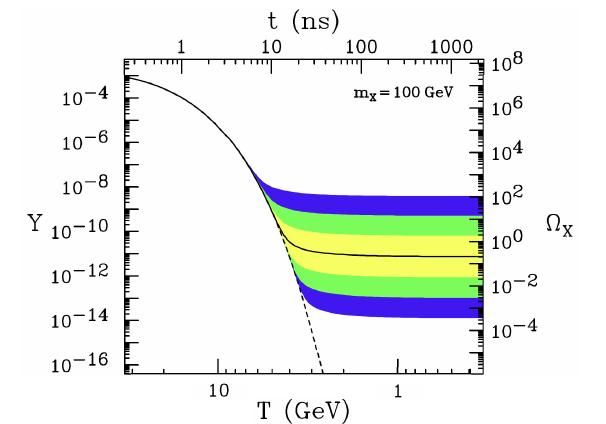
\includegraphics[width=0.75\textwidth]{DarkMatter/Freezeout}
\caption{Evolution of WIMP number density (Y) and resulting thermal relic density (right) as a function of temperature T (bottom) and time
t (top). The solid contour is for an annihilation cross section that yields the correct relic density, and the shaded regions are for cross sections that differr by 10, \SI{e2} and \SI{e3} from this value. The dashed contour is the number density of a particle that remains in thermal equilibrium. This image is taken from \cite{feng:DM}.}
\label{fig:Freezeout}
\end{figure}

Since WIMP DM candidates are particularly well-motivated, a robust experimental effort is underway to either discover DM, or constrain candidate theories. There are two main ways to detect DM which are termed direct and indirect detection, depending on the quest is for DM particles themselves or their annihilation products both discussed in the next section. 

In direct detection searching for WIMPs scattering of nuclei of ordinary matter is involved. Since the nuclear recoil is very small, tipycally \SI{\sim 100}{\kev}, detectors capable capable of low energy detection thresholds, generally located underground, has to be built. The indirect detection involves searches for the products of the very annihilation processes that are responsible for establishing the DM relic density.

All the kind of detection methods are gathered in a Feynman like diagram in \Fig{\ref{fig:detection}}.

\begin{figure}[pt]
\centering
{\fontfamily{pag}\selectfont  
\begin{tikzpicture}
	\draw[thick] (-3,1.5) -- (3,-1.5);
	\draw[thick] (-3,-1.5) -- (3,1.5);
	\filldraw[white] (0,0) circle (0.9cm) ;
	\filldraw[pattern=north east lines] (0,0) circle (0.9cm) ;
	
	\node[left] at (-3,1.5){DM};
	\node[left] at (-3,-1.5){DM};
	\node[right] at (3,1.5){SM};
	\node[right] at (3,-1.5){SM};
	
	\draw[draw=none, fill=orange!80!yellow!70] (-2.5,2)--(2.3,2) -- (2.3,2.2) -- (-2.5,2.2);
	\draw[draw=none, fill=orange!80!yellow!70] (2.2,1.8) -- (2.5,2.1) -- (2.2,2.4) --cycle;
	\node[] at (0,2.9){Indirect detection};
	\node[] at (0,2.5){(Thermal freeze-out)};
	
	\draw[draw=none, fill=yellow!80!red!50] (4,1.3)--(4,-1.1) -- (4.2,-1.1) -- (4.2,1.3);
	\draw[draw=none, fill=yellow!80!red!50] (3.8,-1) -- (4.1,-1.3) -- (4.4,-1) --cycle;
	\node[rotate=-90] at (4.6,0){Direct detection};
	
	\draw[draw=none, fill=orange!80!red!70] (-2.3,-2)--(2.5,-2) -- (2.5,-2.2) -- (-2.3,-2.2);
	\draw[draw=none, fill=orange!80!red!70] (-2.2,-1.8) -- (-2.5,-2.1) -- (-2.2,-2.4) --cycle;
	\node[] at (0,-2.6){Production at colliders};
	
\end{tikzpicture}
}
\caption{Feynman like diagram che ho fatto io which illustrates different methods for dark matter particle detection. The direction of the time axis selects a particular process. In indirect detection Standard Model (SM) particles coming from Dark Matter (DM) decays are revealed.  In direct detction the recoil of nuclei from DM scattering is measured. At colliders SM particles collide to produce a pair of DM candidate.}
\label{fig:detection}
\end{figure}

\subsection{Direct Detection}
The basic idea of Direct Detection is that if our galaxy is populated by WIMPs, a flux of them would run over our detectors and being detected. The WIMP flux on the Earth is estimated to be of the order of \SI{e5}{\per \cm\squared\per\s}. The basic methodology for direct detection experiments is to look for this rare events that might be the signature of WIMP interactions, namely the elastic scattering of a WIMP from a target nucleus~\cite{snowmass}.

This kind of experiments must be carried out underground to reduce the signal contamination from every source of background. This sources comes from cosmic rays, environmental radioactivity or detector radioactivity. For instance, two major experiment ongoing takes place at LNGS, Italy, with the DAMA detector, and the Edelweiss-III experiment at the LSM in Modane, France.

Interaction between WIMPs and nucleon can be spin-dependent when the sign of the scattering amplitude depends on the relative orientation of particle spins, or spin-independent when spin orientations do not affect the amplitude. The spin-independent interaction is expected to be coherent within the entire nucleus, so that if a WIMP has equal coupling to protons and neutrons, the rate scales with the square of the atomic mass of the target nucleus. For spin dependent interactions, the WIMP effectively couples to the net nuclear spin, due to cancellation between opposite spin pairs. It will differ  whether the net nuclear spin is carried by a residual neutron or proton. 

Actual experiments only put upper-limits on WIMPs mass, which can be seen in \Fig{\ref{fig:WIMPcs}} without saying anything else on their nature.

\begin{figure}[pt]
\centering
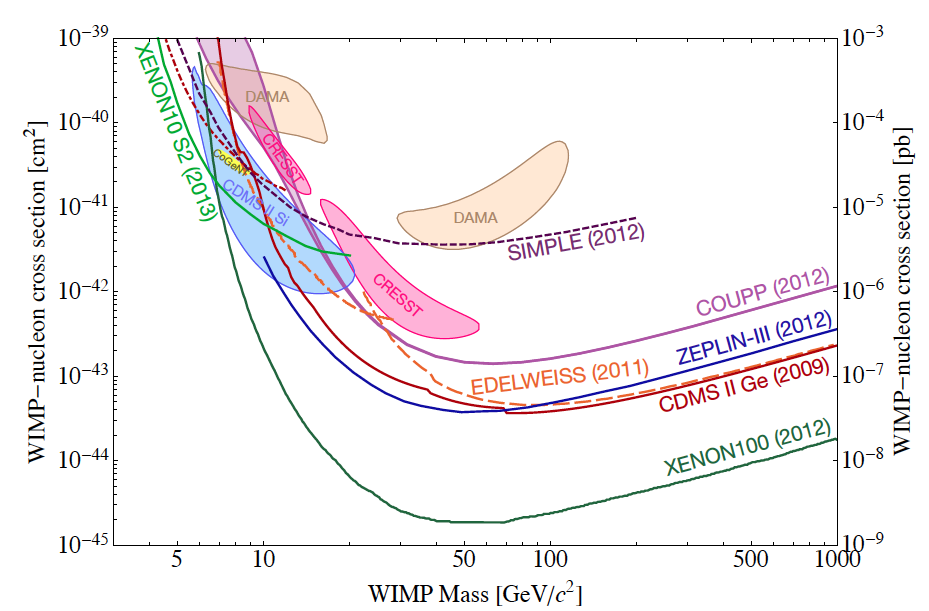
\includegraphics[width=0.8\textwidth]{DarkMatter/WIMPcs}
\caption{Spin-independent WIMP-nucleon cross section limits vs WIMP mass as of summer 2013.}
\label{fig:WIMPcs}
\end{figure}

\subsection{Indirect Detection}
The idea of Indirect Detection is to search for the products of the annihilation processes responsible for establishing the DM relic density which are still going on today. Annihilation probability increase with DM density in a certain region of space and it produces SM particles such gamma rays, neutrinos, electrons, positrons, protons, antiprotons, deuterons, and antideuterons. Therefore WIMPs can be detected by detecting these particles.

The disadvantage associated with Indirect Detection is the background induced by ``ordinary'' astrophysics. If considering only the signal strength from DM annihilations, the best target to detect anihilation products would be the galactic center, but there is a relatively unconstrained astrophysical background to any signals that could be produced there. Many research in the galactic center found signals consistent with DM annihilation but also compatible with the background and statistical fluctuations.

\section{Production at colliders}
Common to all DM searches is the signature of missing transverse momentum (\met) caused by the WIMPs escaping the detector, being produced in association with SM particles. This production share the same idea of direct detection: if a WIMP can scatter from a nucleon, it can be produced in \pp collision at high energy from scattering against SM particles. This result can be pursued in two different ways: we can test a particular model which includes candidates for Dark Matter by checking all the possible decay (as it happens in SUSY physics), on the other hand we can look for it as the only accessible state of a certain process in a model independent way.

These experiments signature is therefore a large value of \met and a back-to-back topology between \met and the Standard Model particle used for tagging. Indeed in order to detect a possible WIMP, it must be tagged with a detectable object. This kind of analisys are called \emph{Mono-X}. They are  characterized by large missing transverse momentum and an energetic particle (the \emph{X}) such a jet (Mono-jet), a photon (\mph) or a \Wboson or \Zboson boson. 

Moreover since DM particle lifetime is extimated to be similar to the Universe, it is long enough to be detected as \met.








